\chapter{Introduction} 
\label{ch:introduction}

A malicious client in a distributed system can undermine the integrity
of the larger distributed application in a number of different ways.
Misbehavior may be the result of a malicious user attempting to either
disrupt services or to gain advantage in a system. For example, a
server application with a vulnerability may be compromised directly by
a modified client. Alternatively, if a client is authoritative for
state data in a larger distributed application, a malicious client may
transmit an illegal version of this state throughout the distributed
application. Real world attacks might consist of a player in a
networked game cheating by modifying the client executable or the user
of a network service might craft a sequence of messages that exploit a
vulnerability in a server application.

There are many techniques for identifying malicious behavior in a
distributed system. Some of these methods include, for example,
probabilistic models of expected traffic patterns, attack signatures
for known vulnerabilities and process level monitoring to identify
control-flow attacks. In this dissertation, however, we address the
problem of identifying malicious clients through the verification
of legitimate client behaviour.

%Classes of Server Vulnerabilities:
%- Common vulnerabilities
%  - Buffer overflows
%- Application specific vulnerabilities
%  - Manipulating client logic
%
%Classes of Client Vulnerabilities:
%- Common vulnerabilities
%  - Buffer overflows
%- Application specific vulnerabilities
%  - Manipulating client logic
%
%
%Attack style and severity:
% - control-data attacks
% - non-control-data attacks

%Validate against a model / signatures
%Compare behavior with statistical models
%Monitor the server, with control flow integrity
%black lists and whitelists

%These methods collect and observe across all levels of
%systems and networking infrastructure; from identifying
%anomolous network traffic patterns using statistical models to
%monitoring stack canaries on server hardware to identify buffer
%overflow attacks. 

Existing techniques for verifying the correctness of client behavior
in distributed applications suffer from imprecision, increased
bandwidth consumption, or significant computational expense. One
approach to defend against client misbehavior is for the server to
validate client messages using a model of client behavior derived from
the sanctioned client software.  For example, Giffin et
al.~\cite{giffin02:remote} and Guha et al.~\cite{guha09:ajax}
developed methods to confirm that requests are consistent with a
control-flow model of the client.  Unfortunately, these approaches may
admit false negatives; compromised clients that make calls consistent
with their control-flow models (but that may still manipulate
application state) can escape detection, in a manner analogous to
mimicry attacks on intrusion-detection
systems~\cite{wagner02:mimicry,tan03:hiding}. In other work, greater
precision has been achieved, but with greater expense.  For example,
the \ripley system~\cite{vikram09:ripley} replays each client on the
server in order to validate the client's requests, but this incurs the
bandwidth overhead of transmitting all client-side inputs (user
inputs, timer values, etc.) to the server to permit replay and the
computational overhead of replaying the client on the server side. 

%A common approach to defend against client misbehavior is for the
%server to validate client messages using a model of valid client
%behavior derived from the sanctioned client software.  For example,
%Giffin et al.~\cite{giffin02:remote} and Guha et
%al.~\cite{guha09:ajax} developed methods to confirm that requests are
%consistent with a control-flow model of the client.  This approach
%admits false negatives, however --- compromised clients that make
%calls consistent with their control-flow models (but that may still
%manipulate application state) can escape detection, in a manner
%analogous to mimicry attacks on intrusion-detection
%systems~\cite{wagner02:mimicry,tan03:hiding}.  Greater precision has
%been achieved, but with greater expense.  For example, the \ripley
%system~\cite{vikram09:ripley} replays each client on the server in
%order to validate the client's requests, but this incurs the bandwidth
%overhead of transmitting all client-side inputs (user inputs, timer
%values, etc.) to the server to
%permit replay and the computational overhead of replaying the client
%on the server side.  An approach by Bethea et
%al.~\cite{bethea11:games} omits transmitting client-side inputs, thus
%not incurring bandwidth overheads, but then must search for whether
%there exist inputs that could have produced the client messages
%observed at the server.  The resulting computational expense renders
%this method of verification useful primarily in an offline fashion
%and, even then, only after modifying test applications to constrain
%the search spaces they present.
%

This \dissertation presents a technique that resolves the tension
between precision, bandwidth consumption and computational expense
with a verification technique that validates legitimate client
behavior as being consistent with the sanctioned client software. We
accomplish behavior verification without encumbering the application
with substantially more bandwidth use and without sacrificing
accuracy. That is, any conclusion reached as to whether the sequence
of client behaviors could, in fact, have been produced from the
sanctioned client software is correct.

\begin{figure}[t]
\centering
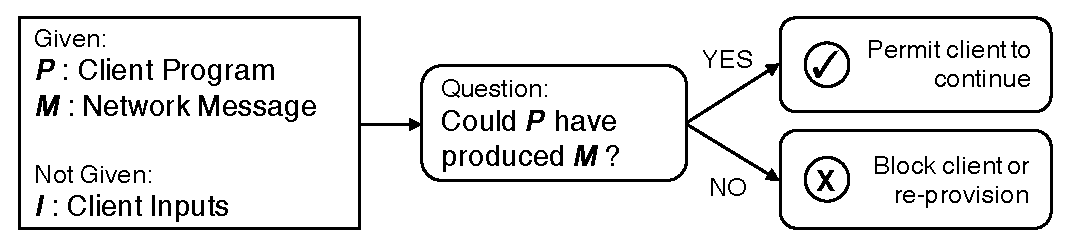
\epsfig{file=figures/introduction/problem.eps, width=0.8\columnwidth}
\caption{Abstracted client verification problem}
\label{fig:intro:prob}
\end{figure}

\section{Problem}
\label{intro:prob}

The client verification problem can be abstracted as follows. A server
wishes to verify that a client is running the sanctioned software, but
does so without modifying the client (e.g., by having the client send
its inputs to the server).  It therefore has no direct access to
client state: the server knows only its own state and the network
messages, $M$, that have been sent.  The problem can then be phrased
as: \emph{Given a client program P, is it possible for P to yield
output $M$?}  This is illustrated in \figref{fig:intro:prob}.

Unfortunately, the general problem of determining whether an arbitrary
program \emph{P} can produce an output \emph{M} is
undecidable~\cite{turing36}.
Fortunately, even though the general problem is undecidable, a
particular instance can be tractable.  The technique that we present
in this dissertation is an application of symbolic
execution~\cite{boyer75:select,king76:symbex}, which has been widely
studied and applied for various purposes.  Dynamic analysis techniques
like symbolic execution typically face scaling challenges as code
complexity and execution length grow, and our case is no exception.
Nevertheless, important advances in the performance of constraint
solving and symbolic execution in the recent past enable our methods
to be viable. In this \dissertation we demonstrate that symbolic
execution can be used as a foundation for verification remote client
behavior.

%In fact, Cochran and Reiter built a tool (using the KLEE symbolic
%execution engine \cite{cadar08:klee}) and demonstrated it on the game
%clients for the 2D games Tetrinet and XPilot.  In these two games,
%the tool can give a ``Yes'' answer quickly enough to verify
%legitimate gameplay in speeds approaching real time.  The ``No''
%answer may be slow, but since client is cheating, such a slowdown is
%acceptable.

%To definitively conclude that a sequence of client messages is
%impossible (the uncommon case), our algorithm incurs a cost similar to
%Bethea et al.'s~\cite{bethea11:games}, however.  As such, we expect
%our algorithm to be useful primarily as an online data reduction
%technique that prunes the client messages that must be logged for
%offline analysis by that (or another) technique.  In addition, clients
%whose messages are not verified quickly by our technique can be
%serviced only provisionally (e.g., with fewer privileges and/or
%logging to enable undoing their effects) while their verification is
%completed offline.

\section{Thesis Statement}
Network messages from a remote client in a distributed system can be
verified using a technique based on symbolic execution, in some cases
at a rate that keeps pace with the application, to determine if the
messages were generated by sanctioned software.

\section{Motivation}

We evaluate our framework in the context of online games.  Online
games provide a useful proving ground for our techniques due to the
frequent manipulation of game clients for the purposes of
cheating~\cite{yan05:classification,lyhyaoui05:categorization,webb08:survey}
and due to the pressure that game developers face to minimize the
bandwidth consumed by their games~\cite{mulligan03:guide}.  As such,
our techniques are directly useful for cheat detection in this domain.
Multi-player online games are very popular and profitable and are
growing more so.  Since 1996 the computer game industry has quadrupled
--- in 2008 alone, worldwide video-game software sales grew 20 percent
to \$32 billion \cite{videobusiness09:sales}.  Estimates place revenue
from online games at \$11 billion, with games such as \wow, which has
more than 10 million subscribers worldwide, bringing in around \$1
billion in revenue for parent company \blizzard
\cite{gamasutra08:wow,gamasutra09:onlinegames}.

Since its inception, the online game industry has been plagued by
cheating of numerous types, in some cases with financial repercussions
to the game operator.  \ageofempires and \americasarmy are examples of
online games that suffered substantial player loss due to
cheating~\cite{spohn:cheating}, and for subscription games, player
loss translates directly to a reduction in revenue.  Game
developers and operators are not the only ones for whom the stakes are
high.  Hoglund and McGraw~\cite{hoglund07:games} argue that ``games
are a harbinger of software security issues to come,'' suggesting that
defenses against game cheats and game-related security problems will
be important techniques for securing future massive distributed
systems of other types.

%\paragraph{Invalid Commands}
The defense that we propose in this \dissertation addresses a class of
malicious behavior that Webb and Soh term {\em invalid commands}:

\begin{quote} {\sl Usually implemented by modifying the game client,
    the invalid command cheat results in the cheater sending commands
    that are not possible with an unmodified game client. Examples
    include giving the cheater's avatar great strength or speed. This
    may also be implemented by modifying the game executable or data
    files. Many games suffer this form of cheating, including console
    games such as \gearsofwar.}~\cite[Section 4.2.3]{webb08:survey}
  \end{quote}

Our technique will detect commands that are invalid in light of the
history of the client's previous behaviors witnessed by the server,
even if those commands could have been valid in some other execution.
Simply put, our approach will detect any client message sequence that
is impossible to observe from the sanctioned client software.


%In this dissertation, we demonstrate our approach with three case
%studies.  First, we apply our technique to the open-source game
%\xpilot.  Because \xpilot was developed as is commonplace today, i.e.,
%with low-level client events being sent to the server, this case study
%does not fully illustrate the strengths of our approach.  However, it
%does demonstrate the (few) ways in which we found it necessary to
%adapt \xpilot to use our technique efficiently.  For the second case
%study, we use a game of our own design that is similar to \pacman but
%that has features to better exercise our technique.  Third, we utilize
%\tetrinet, a multi-player version of \tetris, to demonstrate a client
%that has a much more ambiguity it terms of possible remote client
%states. Together, these case
%studies illustrate the limits and benefits of our approach and serve
%as guidance for game developers who wish to use this technique for
%detecting cheating in their games.
%
%Our strategy exploits the fact that game clients are often structured
%as an event loop that processes user inputs, server messages, or other
%events in the context of current game state and then sends an update
%to the server on the basis of its processing.  We symbolically execute
%the loop to derive a predicate that characterizes the effects of the
%loop, and specifically the update sent to the server, as a function of
%its inputs and game state.  By partially instantiating these
%predicates on the basis of the actual messages the server receives
%from a client and what the server previously sent to the client, a
%{\em \verifier} can then use a constraint solver to determine whether
%the resulting predicate is satisfiable.  If so, then the messages are
%consistent with proper client execution --- i.e., there were {\em
%  some} user inputs that could have yielded these messages.
%
%In our initial work~\cite{bethea11:games}, we developed a verification
%framework that omits transmitting client-side inputs, thus not
%incurring bandwidth overheads, but then must search for whether there
%exist inputs that could have produced the client messages observed at
%the server.  The resulting computational expense renders this method
%of verification useful primarily in an offline fashion and only after
%modifying test applications to constrain the search spaces they
%present.
%
%In our follow-up work~\cite{cochran13:toward}, we demonstrated an
%extension to the aforementioned approach~\cite{bethea11:games} with
%several advances to achieve further progress. The extended
%client-checking algorithm that we proposed retains precision while
%permitting better tradeoffs between bandwidth costs and computational
%expense in the common case of a legitimate client. First, we augment
%our verification algorithm to use a training phase to build baselines
%of client behavior to use in prioritizing paths to search during
%verification. This approach completes verification much more
%efficiently in the common case of a legitimate client.  Second, we
%experimented with a framework that allows the client software to be
%instrumented, so that in its messages, the running client will convey
%"hints" that can aid verification. Such configurations that allow
%minimal additional bandwidth, complete verification even faster in the
%common case of a legitimate client. To definitively conclude that a
%sequence of client messages is impossible (the uncommon case), these
%extensions to our algorithm do not necessarily provide a performance
%benefit because all feasible paths must be exhaustively searched.  As
%such, the current state of our algorithm is useful as a data reduction
%technique that prunes the client messages that must be logged for
%offline analysis by that (or another) technique.  Clients whose
%messages are not verified quickly by our technique can be serviced
%only provisionally (e.g., with fewer privileges and/or logging to
%enable undoing their effects) while their verification is completed
%offline.
%
%We have planned several extensions to the current framework. First, is
%improved modeling of environment interactions to enable support of
%more complex applications. Networked multiplayer games are an
%excellent domain for our technique, but we believe with better
%application support, we can expand the reach of our framework. Second,
%we believe we can push the limits of current symbolic execution
%performance by minimizing the overhead of interpreting non-symbolic
%instructions and with extensions to the symbolic execution engine
%(\klee) to utilize multi-core processors. Taken together, our
%improvements open the door to novel uses of behavior verification,
%including doing so in an online fashion alongside servicing client
%requests.
%
%%\subsection{Buggy Server Code}
%%\subsection{Internet of Things}
%%\subsection{Cheating in Online Games}
%%\subsection{Complex Input Validation}
%
%%\subsection{Using Testing Tools for Verification}
%%\subsection{Symbolic Client Verification}
%%\subsection{Limitations}
%%\subsection{Advantages}
%%\section{Summary}

%\section{tissec introduction}
%\label{sec:intro}

%Multi-player online games are very popular and profitable and are
%growing more so.  Since 1996 the computer game industry has quadrupled
%--- in 2008 alone, worldwide video-game software sales grew 20 percent
%to \$32 billion \cite{videobusiness09:sales}.  Estimates place revenue
%from online games at \$11 billion, with games such as \wow, which has
%more than 10 million subscribers worldwide, bringing in around \$1
%billion in revenue for parent company \blizzard
%\cite{gamasutra08:wow,gamasutra09:onlinegames}.
%
%Since its inception, the online game industry has been plagued by
%cheating of numerous types, in some cases with financial repercussions
%to the game operator.  \ageofempires and \americasarmy are examples of
%online games that suffered substantial player loss due to
%cheating~\cite{spohn:cheating}, and for subscription games, player
%loss translates directly to a reduction in revenue.  And game
%developers and operators are not the only ones for whom the stakes are
%high.  Hoglund and McGraw~\cite{hoglund07:games} argue that ``games
%are a harbinger of software security issues to come,'' suggesting that
%defenses against game cheats and game-related security problems will
%be important techniques for securing future massive distributed
%systems of other types.
%
%In this \dissertation, we develop an approach to detect a significant class of
%cheats in which a player changes a game client to allow behaviors that
%a sanctioned game client would not allow.  To accomplish this, the
%player might modify the client executable or in-memory data structures
%of a running client, for example.  Today, the most robust defense
%against such client modification is to maintain authoritative state at
%the server, beyond the reach of direct manipulation by cheaters.  This
%defense, however, exacts a heavy price from game operators, owing to
%the increased bandwidth use that results from sending low-level
%client events (in the limit, every player input) to the server for
%accessing such state and conveying the effects back to clients.  As
%bandwidth is one of the largest costs for large-scale game
%operators~\cite{mulligan03:guide} and also a recurring one, this
%tension between bandwidth use and cheat prevention is problematic:
%\begin{quote}
%{\sl In the US and European markets, a good goal to shoot for is 4-6
%kilobits per second (kps)/player or less. ... If you can get the bit
%rate down to 2kps, you're ``golden.''  It's hard to see how that can
%happen, however, without putting dangerous amounts of data directly
%into the client, which is just asking for trouble from talented
%cheaters and hackers.}~\cite[p.~112]{mulligan03:guide}
%\end{quote}
%The movement of games to all manners of devices using wireless,
%volume-priced communication only reinforces the importance
%of keeping bandwidth utilization to a minimum.  Moreover, even with
%the amount of detailed client information collected at the server,
%server-side checking today is heuristic (and thus potentially
%incomplete) and manually programmed (and thus effort-intensive):
%\begin{quote}
%{\sl Players love to cheat --- especially in online games ... be
%ready to add server-side support to prevent user cheating with
%methods that you were not able to predict.}~\cite{hawkins03:quote}
%\end{quote}
%
%In this paper we demonstrate a technique to detect any type of
%cheating that causes the client to exhibit behavior, as seen by the
%server, that is inconsistent with the sanctioned client software and
%the game state known at the server.  That is, our approach discerns
%whether there was {\em any possible sequence} of user inputs to the
%sanctioned client software that could have given rise to each message
%received at the server, given what the server knew about the game
%client based on previous messages from the client and the messages the
%server sent to the client. In doing so, our approach remedies the
%previously heuristic and manual construction of server-side checks.
%Moreover, our approach potentially enables new game designs that
%reduce bandwidth use by placing more authoritative state at the
%client, since our approach verifies that the client's behavior is
%consistent with legal management of that state.  While reducing
%interaction with the client will generally increase the computational
%cost of our verification, verification need not be done on the
%critical path of game play and can be performed selectively (e.g.,
%only for suspected or winning players).  Moreover, it can benefit from
%the dramatic growth of inexpensive computing power (larger numbers of
%cores) in game-operator server farms.
%
%Our strategy exploits the fact that game clients are often structured
%as an event loop that processes user inputs, server messages, or other
%events in the context of current game state and then sends an update
%to the server on the basis of its processing.  We symbolically execute
%the loop to derive a predicate that characterizes the effects of the
%loop, and specifically the update sent to the server, as a function of
%its inputs and game state.  By partially instantiating these
%predicates on the basis of the actual messages the server receives
%from a client and what the server previously sent to the client, a
%{\em \verifier} can then use a constraint solver to determine whether
%the resulting predicate is satisfiable.  If so, then the messages are
%consistent with proper client execution --- i.e., there were {\em
%  some} user inputs that could have yielded these messages.
%
%We demonstrate our approach with three case studies.  First, we
%apply our technique to the open-source game \xpilot.  Because \xpilot
%was developed as is commonplace today, i.e., with low-level client
%events being sent to the server, this case study does not fully
%illustrate the strengths of our approach.  However, it does
%demonstrate the (few) ways in which we found it necessary to adapt
%\xpilot to use our technique efficiently.  For the second case study,
%we use a game of our own design that is similar to \pacman but that
%has features to better exercise our technique.  Third, we utilize
%\tetrinet, a multiplayer version of \tetris, to demonstrate the
%bandwidth savings that our approach can enable.  Together, these case
%studies illustrate the limits and benefits of our approach and serve
%as guidance for game developers who wish to use this technique for
%detecting cheating in their games.
%
%Following our initial investigation of these case studies, we
%investigate the impact of message loss on our verification technique.
%We extend our technique to improve verification performance in the
%face of message loss on the network.  We then evaluate this extension
%using \xpilot, since it is an example of a game built to use an
%unreliable transport protocol for performance reasons and consequently
%to continue gameplay despite message loss.
%
%\section{ndss13 Introduction}
%\label{sec:intro}
%
%In client-server applications, client misbehavior can pose dangers to
%the larger distributed application in a variety of ways.  A
%manipulated client may be able to compromise the server directly if
%the server has an extant vulnerability.  Even if the server has no
%such vulnerabilities, any application state for which the client is
%authoritative can be altered by a misbehaving client and then
%propagated via the server to the larger distributed application.
%
%A common approach to defend against client misbehavior is for the
%server to validate client messages using a model of valid client
%behavior derived from the sanctioned client software.  For example,
%Giffin et al.~\cite{giffin02:remote} and Guha et
%al.~\cite{guha09:ajax} developed methods to confirm that requests are
%consistent with a control-flow model of the client.  This approach
%admits false negatives, however --- compromised clients that make
%calls consistent with their control-flow models (but that may still
%manipulate application state) can escape detection, in a manner
%analogous to mimicry attacks on intrusion-detection
%systems~\cite{wagner02:mimicry,tan03:hiding}.  Greater precision has
%been achieved, but with greater expense.  For example, the \ripley
%system~\cite{vikram09:ripley} replays each client on the server in
%order to validate the client's requests, but this incurs the bandwidth
%overhead of transmitting all client-side inputs (user inputs, timer
%values, etc.) to the server to
%permit replay and the computational overhead of replaying the client
%on the server side.  An approach by Bethea et
%al.~\cite{bethea11:games} omits transmitting client-side inputs, thus
%not incurring bandwidth overheads, but then must search for whether
%there exist inputs that could have produced the client messages
%observed at the server.  The resulting computational expense renders
%this method of verification useful primarily in an offline fashion
%and, even then, only after modifying test applications to constrain
%the search spaces they present.
%
%In this \dissertation we develop a client-checking algorithm that retains
%precision while permitting better tradeoffs between bandwidth costs
%and computational expense in the common case of a legitimate client.
%Our algorithm builds from the aforementioned approach of Bethea et
%al.~\cite{bethea11:games} but exploits a training phase to guide a
%search for a path through the client program that could have produced
%a message observed at the server.  One configuration of our algorithm
%incurs no additional bandwidth costs, like Bethea et al.'s, but
%completes verification much more efficiently in the common case of a
%legitimate client.  Another configuration of our algorithm consumes
%minimal additional bandwidth --- in our tests, at most two bytes per
%client-to-server message --- and completes verification even faster in
%the common case of a legitimate client.  Moreover, we reiterate that
%our algorithm is precise in the sense of having no false negatives and
%no false positives.  That is, any sequence of client messages that our
%technique declares legitimate actually is, in the sense that there
%exist inputs that would have driven the sanctioned client software to
%send that sequence of messages,\footnote{More precisely, the only
%source of false negatives is the fidelity of modeling values returned
%by components with which the client software interacts (e.g., the
%client OS).  This will be discussed further in \secref{sec:eval}.} and
%any sequence of client messages that our technique declares impossible
%is actually inconsistent with the client software.
%
%To definitively conclude that a sequence of client messages is
%impossible (the uncommon case), our algorithm incurs a cost similar to
%Bethea et al.'s~\cite{bethea11:games}, however.  As such, we expect
%our algorithm to be useful primarily as an online data reduction
%technique that prunes the client messages that must be logged for
%offline analysis by that (or another) technique.  In addition, clients
%whose messages are not verified quickly by our technique can be
%serviced only provisionally (e.g., with fewer privileges and/or
%logging to enable undoing their effects) while their verification is
%completed offline.
%
%We evaluate our algorithm in the context of online games.  Online
%games provide a useful proving ground for our techniques due to the
%frequent manipulation of game clients for the purposes of
%cheating~\cite{yan05:classification,lyhyaoui05:categorization,webb08:survey}
%and due to the pressure that game developers face to minimize the
%bandwidth consumed by their games~\cite{mulligan03:guide}.  As such,
%our techniques are directly useful for cheat detection in this domain.
%Moreover, Hoglund and McGraw~\cite{hoglund07:games} argue that ``games
%are a harbinger of software security issues to come,'' suggesting that
%defenses against game cheats and game-related security problems will
%be important techniques for securing future massive distributed
%systems of other types.  Our evaluations show, for example, that
%verifying the behavior of a valid client in the \tetrinet game can
%often keep up with the pace of gameplay.  Moreover, our algorithm
%succeeds in verifying messages traces of the highly interactive
%\xpilot game without game restrictions required by previous
%techniques~\cite{bethea11:games}.
%
%The technique that we develop here is an application of symbolic
%execution~\cite{boyer75:select}, which has been widely studied and
%applied for various purposes (see \secref{sec:related}).  Dynamic
%analysis techniques like symbolic execution typically face scaling
%challenges as code complexity and execution length grow, and our case
%is no exception.  We believe that the technique we develop here to
%prioritize path analysis on the basis of historical usage may be more
%broadly useful, i.e., outside of behavior verification in distributed
%systems, to contain the expense of dynamic analysis.
%
%The rest of this \dissertation is structured as follows.  We discuss related
%work in \secref{sec:related} and necessary background in
%\secref{sec:goals}.  We present our algorithm in \secref{sec:training}
%and \secref{sec:verification}.  Evaluation results for this algorithm
%are presented in \secref{sec:eval}, and we conclude in
%\secref{sec:conclusion}.
%
%
%

%In our initial work~\cite{bethea11:games}, we developed a verification
%framework that omits transmitting client-side inputs, thus not
%incurring bandwidth overheads, but then must search for whether there
%exist inputs that could have produced the client messages observed at
%the server.  The resulting computational expense renders this method
%of verification useful primarily in an offline fashion and only after
%modifying test applications to constrain the search spaces they
%present.
%
%In our follow-up work~\cite{cochran13:toward}, we demonstrated an
%extension to the aforementioned approach~\cite{bethea11:games} with
%several advances to achieve further progress. The extended
%client-checking algorithm that we proposed retains precision while
%permitting better tradeoffs between bandwidth costs and computational
%expense in the common case of a legitimate client. First, we augment
%our verification algorithm to use a training phase to build baselines
%of client behavior to use in prioritizing paths to search during
%verification. This approach completes verification much more
%efficiently in the common case of a legitimate client.  Second, we
%experimented with a framework that allows the client software to be
%instrumented, so that in its messages, the running client will convey
%"hints" that can aid verification. Such configurations that allow
%minimal additional bandwidth, complete verification even faster in the
%common case of a legitimate client. To definitively conclude that a
%sequence of client messages is impossible (the uncommon case), these
%extensions to our algorithm do not necessarily provide a performance
%benefit because all feasible paths must be exhaustively searched.  As
%such, the current state of our algorithm is useful as a data reduction
%technique that prunes the client messages that must be logged for
%offline analysis by that (or another) technique.  Clients whose
%messages are not verified quickly by our technique can be serviced
%only provisionally (e.g., with fewer privileges and/or logging to
%enable undoing their effects) while their verification is completed
%offline.
%

\section{Contributions}
The key contributions of this dissertation are:

\begin{itemize}

\item A novel technique, \textit{symbolic client verification}, that
  can verify the behavior of a remote client by determining whether a
  sequence of messages from a remote client could have been generated
  by sanctioned software.

\item An extension of symbolic client verification to optimize
  identification of legitimate clients that uses training data to
  improve performance.

\item A parallel algorithm for symbolic client verification that
  significantly improves performance.

\item Evaluations of symbolic client verification in the framework of
  online games on a game of our own design, called \capman, and two
  real-world games, \xpilot and \tetrinet.

%\item We have demonstrated two techniques that use symbolic execution
%  to verify whether a sequence of messages from a remote client could
%  have been generated by the sanctioned software.
%
%\item We have investigated the feasibility of using our technique to
%  reduce the bandwidth consumption of a multiplayer
%  game~\cite{bethea11:games}.
%
%\item We have demonstrated an effective technique to improve the path
%  selection heuristic in our verification framework by selecting paths
%  to search first based on execution history~\cite{cochran13:toward}.
%
%\item We have parallelized core components of our framework, including
%  the \klee symbolic execution tool (\chref{ch:par}).

\end{itemize}

The rest of this dissertation is outlined as follows. \chref{ch:background}
gives an overview of symbolic execution and related work.
\chref{ch:scv} introduces symbolic client verification along with
an evaluation in the context of online games.
\chref{ch:scv} is based on work that appears in the proceedings of the
17th ISOC Network and Distributed System Security
Symposium~\cite{bethea10:games} and
in the ACM Transactions on Information and System
Security~\cite{bethea11:games}.
\chref{ch:guided} presents
an optimistic version of symbolic client verification that prioritizes
legitimate clients and also provides an evaluation.
\chref{ch:guided} is based on work published in the
proceedings of
the 20th ISOC Network and Distributed System Security
Symposium~\cite{cochran13:toward}.
\chref{ch:par}
presents a parallel algorithm for symbolic client verification and
demonstrates the improvements it provides with an evaluation on
verification of legitimate client in the context of online games.
Portions of \chref{ch:par} have been published in a technical report~\cite{chi16:crypto}.
\chref{ch:conclusion} concludes the dissertation.

